\documentclass[a4paper,12pt]{scrartcl}
\usepackage[utf8]{inputenc}
\usepackage[UKenglish]{isodate}
\usepackage{csquotes}
\usepackage{graphicx}
\usepackage{wrapfig}
\usepackage{enumitem}
\usepackage{pdflscape}
\usepackage[toc,page]{appendix}
\usepackage{geometry}
\usepackage{hyperref}
\usepackage{cleveref}
\usepackage{listings}
\usepackage{csvsimple}
\usepackage{booktabs}
\usepackage{longtable}
\usepackage{caption}
\usepackage{subcaption}
\usepackage[colorinlistoftodos]{todonotes}
\usepackage[british]{babel}
\usepackage{float}
%\usepackage[margin=1in]{geometry}
\usepackage{listings}
\usepackage{color}
 
\definecolor{codegreen}{rgb}{0,0.6,0}
\definecolor{codegray}{rgb}{0.5,0.5,0.5}
\definecolor{codepurple}{rgb}{0.58,0,0.82}
\definecolor{backcolour}{rgb}{0.95,0.95,0.92}
 
\lstdefinestyle{mystyle}{
	language=PHP,
    backgroundcolor=\color{backcolour},   
    commentstyle=\color{codegray},
    keywordstyle=\color{magenta},
    numberstyle=\tiny\color{codegray},
    stringstyle=\color{codegreen},
    basicstyle=\footnotesize,
    breakatwhitespace=false,         
    breaklines=true,                 
    captionpos=b,                    
    keepspaces=true,                 
    numbers=left,                    
    numbersep=5pt,                  
    showspaces=false,                
    showstringspaces=false,
    showtabs=false,                  
    tabsize=3,
    morekeywords={ new, __halt_compiler, abstract, and, array, as, break, callable, case, catch, class, clone, const, continue, declare, default, die, do, echo, else, elseif, empty, enddeclare, endfor, endforeach, endif, endswitch, endwhile, eval, exit, extends, final, for, foreach, function, global, goto, if, implements, include, include_once, instanceof, insteadof, interface, isset, list, namespace, new, or, print, private, protected, public, require, require_once, return, static, switch, throw, trait, try, unset, use, var, while, xor}
}

\lstset{language=Java,
  showspaces=false,
  showtabs=false,
  breaklines=true,
  showstringspaces=false,
  breakatwhitespace=true,
  commentstyle=\color{pgreen},
  keywordstyle=\color{pblue},
  stringstyle=\color{pred},
  basicstyle=\ttfamily,
  moredelim=[il][\textcolor{pgrey}]{$$},
  moredelim=[is][\textcolor{pgrey}]{\%\%}{\%\%}
}
 
\lstset{style=mystyle}

\graphicspath{ {images/} }
\usepackage[
	backend=biber,
	style=ieee,
	]{biblatex}

\addbibresource{references.bib}

\title{829H1 Real-Time Embedded Systems Exercise 4}
\author{Candidate No: 105936}
\date{\today}

\begin{document}
	
	\begin{titlepage}
		\maketitle
	\end{titlepage}
	
	\tableofcontents
	\newpage
	
	\section{Introduction}
	{
		This report focuses on using serial communications on the board and shows the work completed during the laboratory sessions and what was learnt. Code listings for some of the created programs can be found in \cref{Appendix:start}.
	}
	
	\section{Experiments}
	{
		\subsection{Serial Communications}
		{
			For this experiment I created a SPI master object which allowed me to output data using serial methods on three pins, these pins were PTD2 which was the MOSI, PTD3 the MISO and PTD1 which was the clock. 
			\begin{figure}[h]
				\centering
				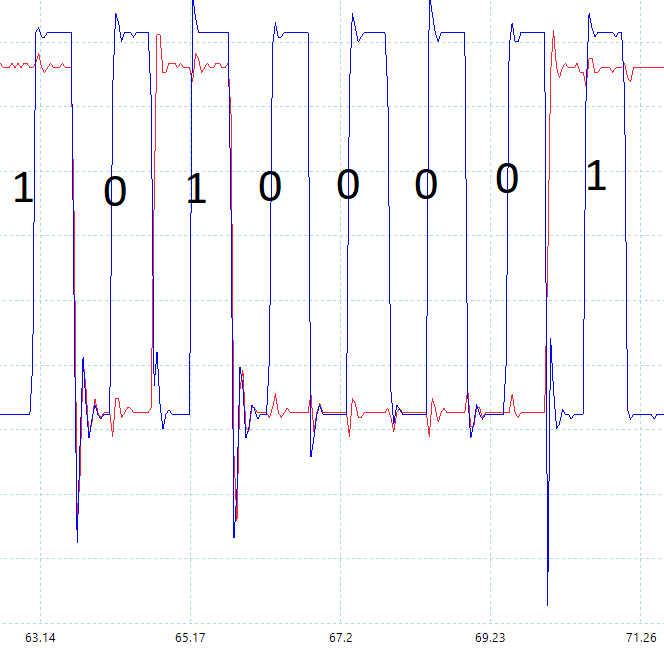
\includegraphics[width=0.5\textwidth]{Ex1/Task1-Edited}
				\caption{An Image showing the output on the oscilloscope when running code from \cref{appendix:ex1-1}}
				\label{img:Ex1-Task1}
			\end{figure}
			\cref{img:Ex1-Task1} demonstrates the output of sending a word out using serial communication. Here the blue line represents the clock and red the signals.
			
			\subsubsection{Using Different SPI Modes}
			{
				This changes the clock signal as shown in \cref{img:ClockMode0}, \cref{img:ClockMode1}, \cref{img:ClockMode2} and \cref{img:ClockMode3}.
				\begin{figure}[h]
					\centering
					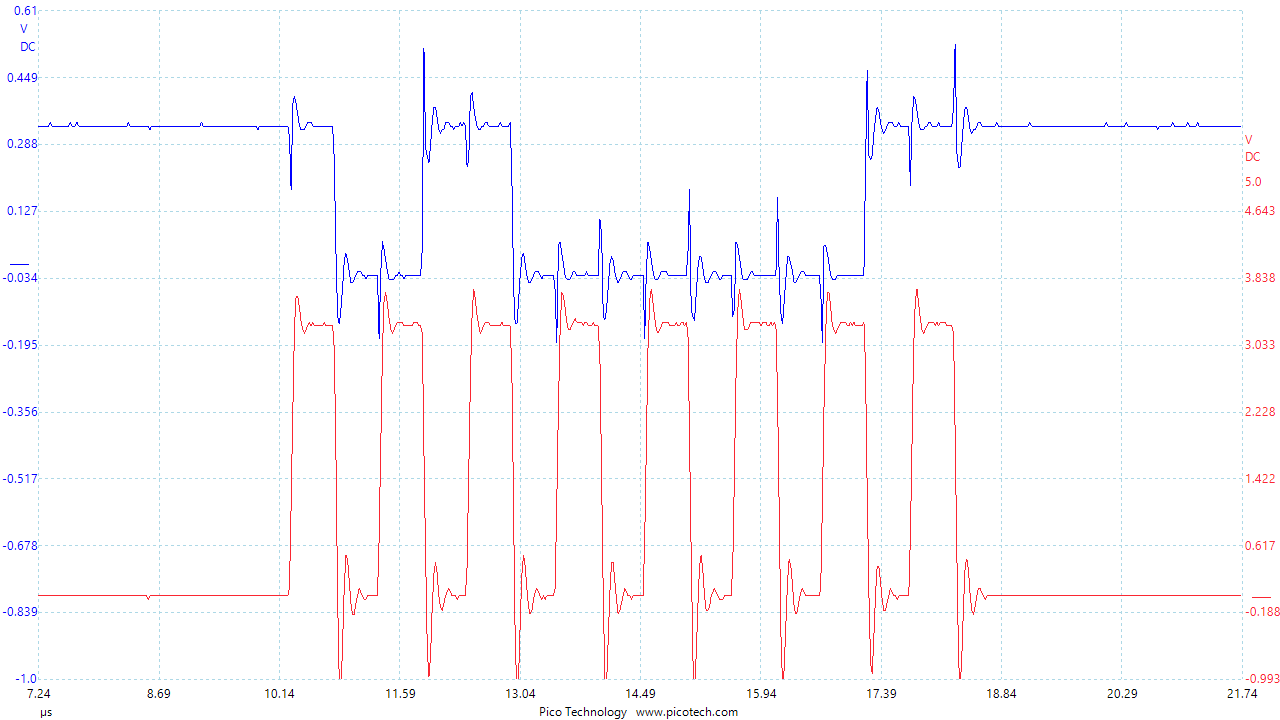
\includegraphics[width=\textwidth]{Ex1/mode0}
					\caption{This figure shows clock mode 0 please note that the red is the clock and blue is the word being transmitted}
					\label{img:ClockMode0}
				\end{figure}
				\begin{figure}[h]
					\centering
					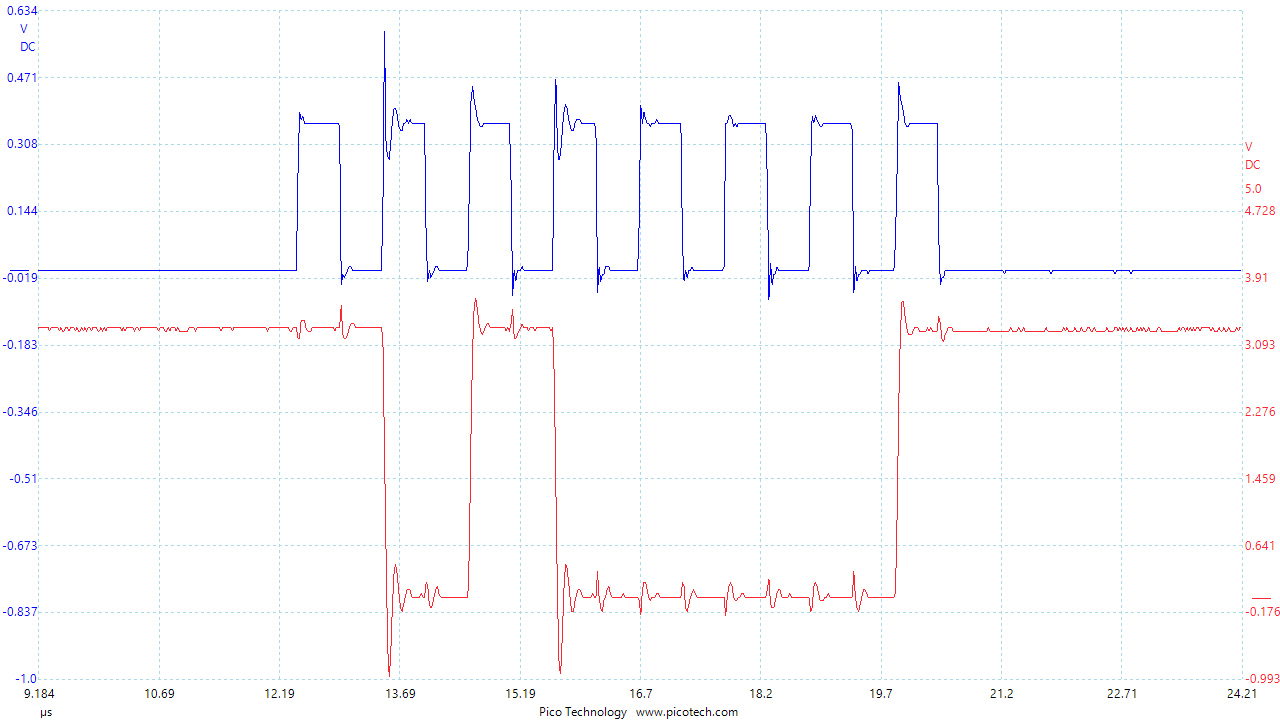
\includegraphics[width=\textwidth]{Ex1/mode1}
					\caption{This shows clock mode 1}
					\label{img:ClockMode1}
				\end{figure}
				\begin{figure}[h]
					\centering
					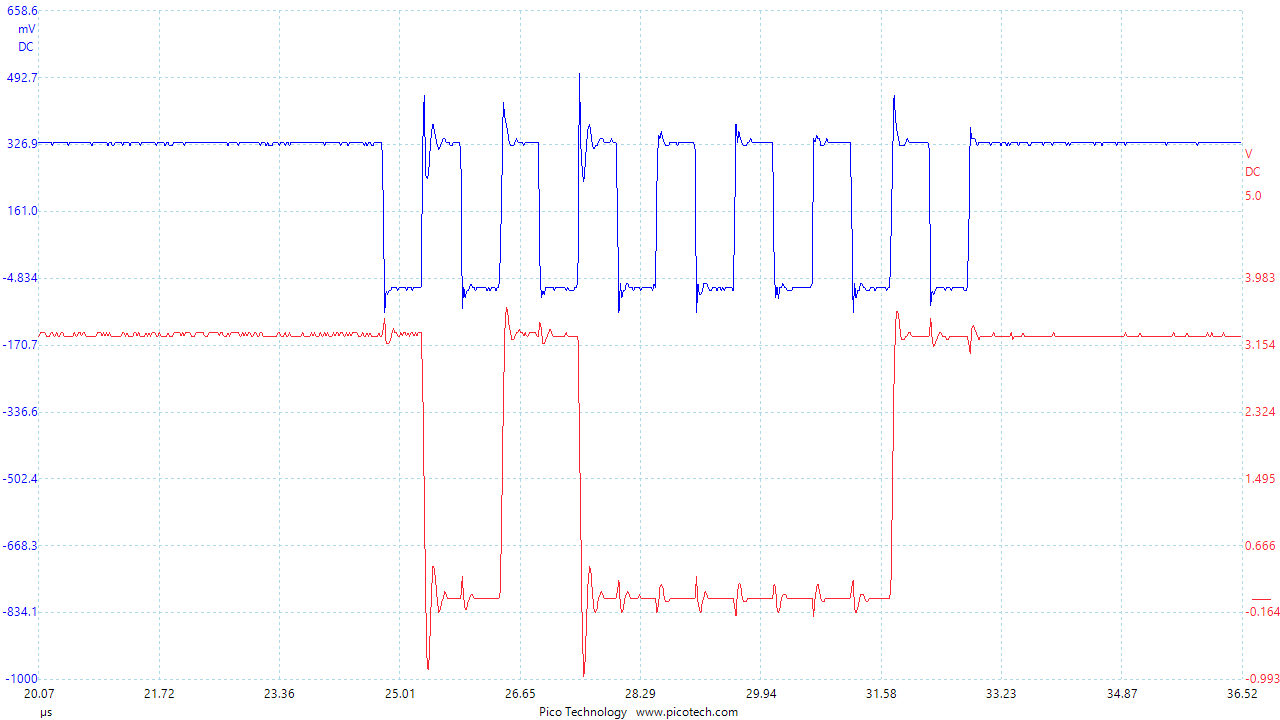
\includegraphics[width=\textwidth]{Ex1/mode2}
					\caption{This shows clock mode 2}
					\label{img:ClockMode2}
				\end{figure}
				\begin{figure}[h]
					\centering
					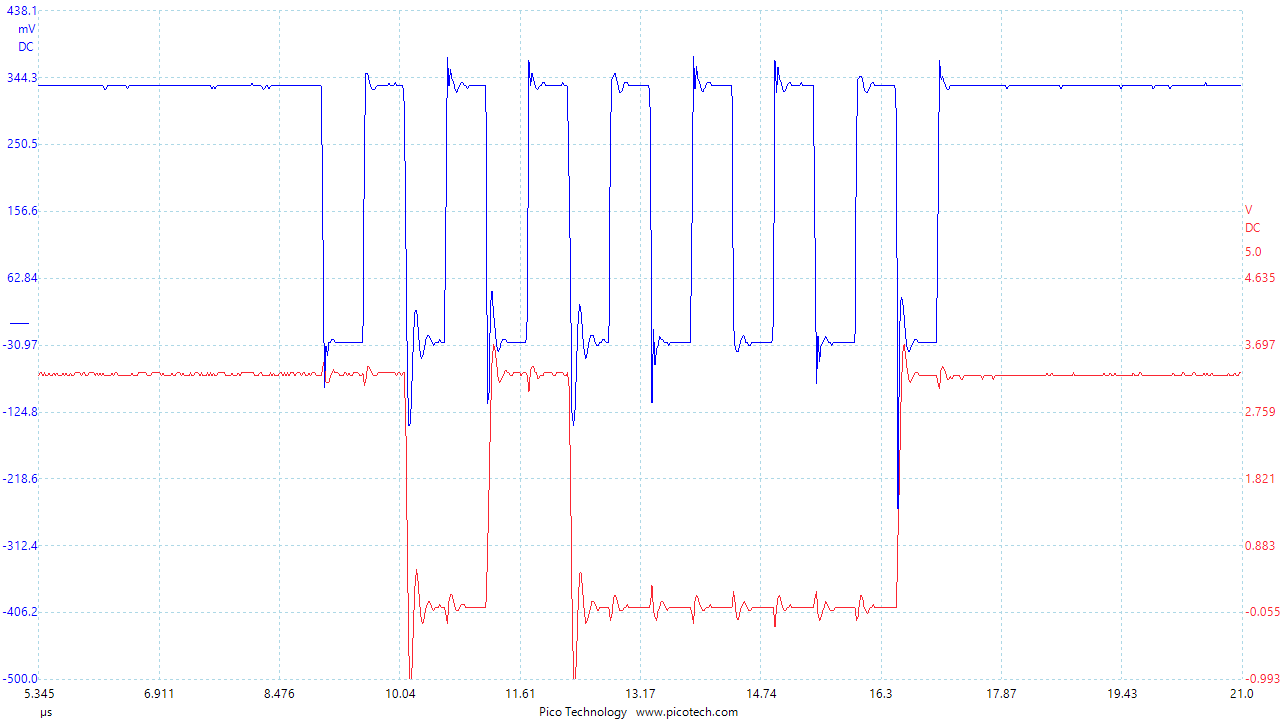
\includegraphics[width=\textwidth]{Ex1/mode3}
					\caption{This shows clock mode 3}
					\label{img:ClockMode3}
				\end{figure}
				As you can see from the graphs the same word is being transmitted in each configuration. However, the clock signal is changing. This is because we are changing the clock mode through the different phases of the signal.
			}
		
			\subsubsection{Using a Different Number of bits}
			{
				The code for 12-bit operation can be found in \cref{appendix:ex1-2}. I am now sending the binary number 100010100001 this is equivalent to 0x8A1 or 2209 in decimal. The oscilloscope output for this can be seen in \cref{img:12bit0x8a1}. The figure clearly shows that more bits are being transmitted per word and if you read the values you can see it's transmitting correctly.
				\begin{figure}[h]
					\centering
					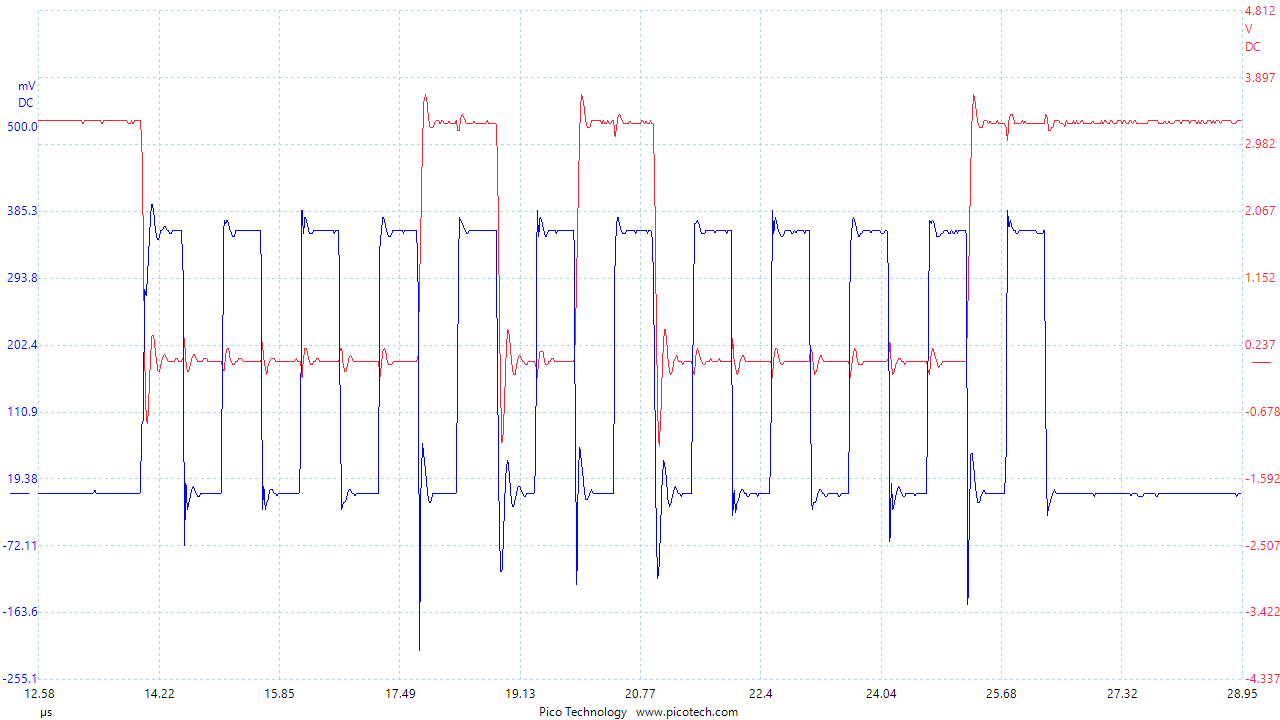
\includegraphics[width=\textwidth]{Ex1/12bit0x8a1}
					\caption{This shows 0x8A1 being transmitted as 12 bits with clock mode 0}
					\label{img:12bit0x8a1}
				\end{figure}
				I also attempted to display a 16-bit word this was 0x8AA1 or 1000101010100001 in binary this can be seen in \cref{img:16bit0x8aa1} and the code can be found in \cref{appendix:ex1-3}.
				\begin{figure}[h]
					\centering
					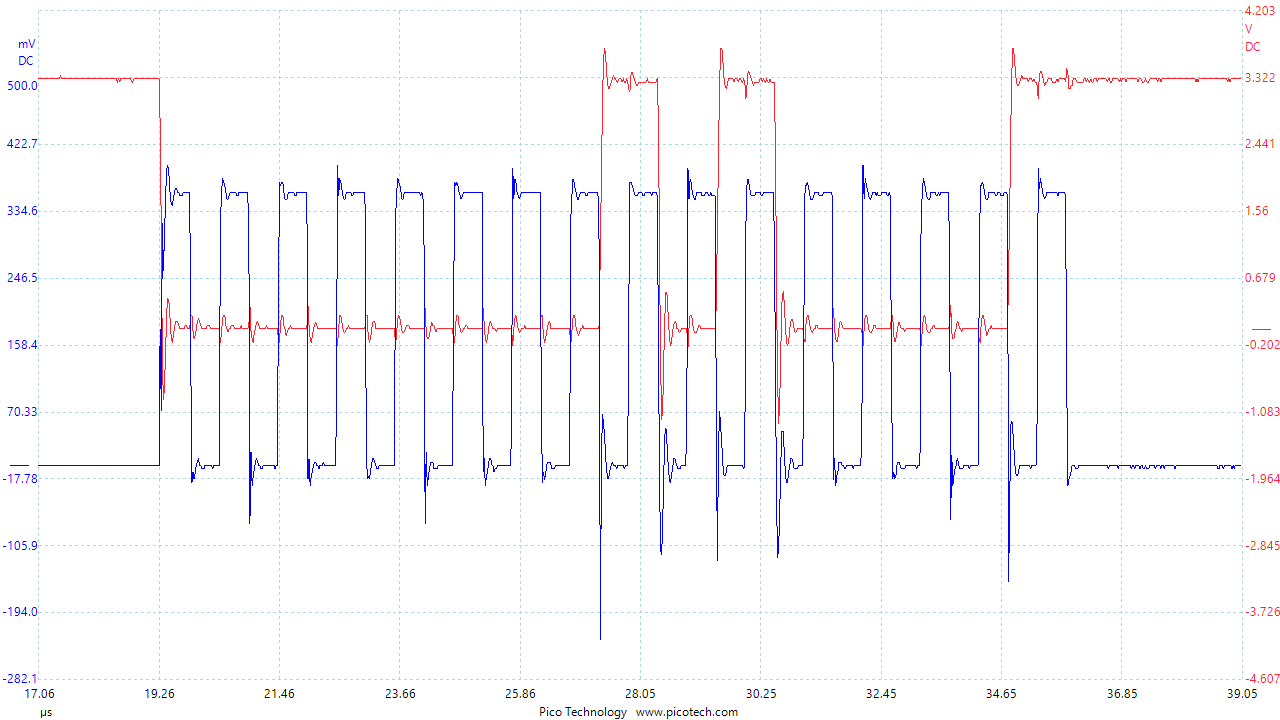
\includegraphics[width=\textwidth]{Ex1/16bit0x8aa1}
					\caption{This shows 0x8AA1 being transmitted as 16 bits with clock mode 0}
					\label{img:16bit0x8aa1}
				\end{figure}
			}
		}
		\subsection{Linking Two Boards together}
		{
			This requires the use of a master and slave program the master program allows a slave to be attached to the board using the outputs. It sends a word to the slave board and gets a reply and sets the LEDs accordingly. The slave program receives a word from the master and sets the LEDs accordingly then sends a word back depending on the switch position code for these two programs can be found in \cref{appendix:ex2}. This is an example of a serial connection as we have the clock and two data lines one for input and one for output.
			
			\subsubsection{What happens when MOSI is disconnected}
			{
				When the master output/slave input is disconnected the master board still lights up this is because the slave output line is still connected therefore as the master does not know that it is not transmitting it assumes the system is still working correctly. Also, the clock line is still connected so the slave knows when and how to transmit back.
				
			}
			\subsubsection{What happens when MISO is disconnected}
			{
				When the master input/slave output is disconnected nothing works this is a bit of a surprise to me as I expected the master to still be able to control the slave's lights. as the slave is still receiving the master's output.
			}
			\subsubsection{What happens when clock is disconnected}
			{
				When the clock line is disconnected none of the functions work this is because the slave is not able to tell where one bit ends, and another begins and it also does not know how to send the data back to the master.
			}
			\subsubsection{What happens when the slave select/chip select is removed?}
			{
				When the slave/chip select line is removed again none of the functions work this is because the SPI library system we are using requires this line to be connected.5
			}
		}
		\subsection{USB}
		{
			This implements a simple program where the computers mouse is moved on each iteration of the for loop this allows us to test that the USBMouse library is working properly the code for this can be found at \cref{appendix:ex3-1}.
			\subsubsection{Page Scroller}
			{
				This is another simple program which when run simply continuously scrolls to the bottom of the page. Code for this can be found in \cref{appendix:ex3-2}.
			}
			\subsubsection{Mouse Buttons}
			{
				For this task I had to use knowledge I gained from earlier exercises. Therefore, I added interrupts on the switches which called the \lstinline|USBMouse.press()| and \lstinline|USBMouse.release()| the code for this can be found in \cref{appendix:ex3-3}.
			}
			\subsubsection{Accelerometer Mouse}
			{
				For this task I had to use an additional library to access the accelerometer data. I used the FXOS8700Q\cite{accelLib} library. I then needed to use these values in the accelerator data to make the mouse move, the code for this can be found in \cref{appendix:ex3-4}.
			}
		}
	}
	\section{Conclusion}
	{
		In conclusion, this was a useful exercise on using serial communications and then learning how to use the USBDevice functions and also how to use the accelerometer values. I would have liked to go on and use the joystick to control the mouse however I ran out of time.
	}
	
	\newpage
	\begin{appendices}
	\label{Appendix:start}
	\section{Lab Exercise 1}
	{
		\subsection{Part 1}
		{
			\label{appendix:ex1-1}
			\lstinputlisting[language=c++]{CodeListings/Ex1/mainPart1.cpp}
		}
		\subsection{Part 2}
		{
			\label{appendix:ex1-2}
			\lstinputlisting[language=c++]{CodeListings/Ex1/mainPart2.cpp}
		}
		\subsection{Part 3}
		{
			\label{appendix:ex1-3}
			\lstinputlisting[language=c++]{CodeListings/Ex1/mainPart3.cpp}
		}
	}
	\section{Lab Exercise 2}
	{
		\label{appendix:ex2}
		\subsection{Part 1 - Master Program}
		{
			\label{appendix:ex2-1}
			\lstinputlisting[language=c++]{CodeListings/Ex2/main-master.cpp}
		}
		\subsection{Part 2 - Slave Program}
		{
			\label{appendix:ex2-2}
			\lstinputlisting[language=c++]{CodeListings/Ex2/main-slave.cpp}
		}
	}

\end{appendices}
	\printbibliography[heading=bibintoc,title=References]
\end{document}
